\documentclass[tikz, border = 5pt]{standalone}

\begin{document}
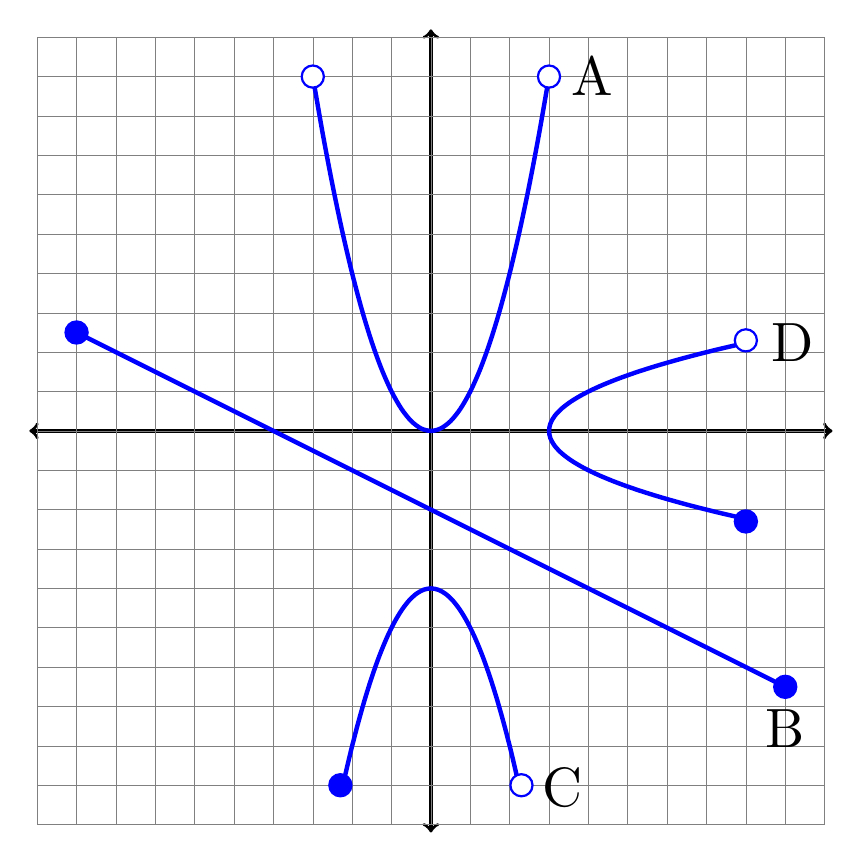
\begin{tikzpicture}
  % axis
  \draw[very thick, <->] (0, -5.1) -- (0, 5.1);
  \draw[very thick, <->] (-5.1, 0) -- (5.1, 0);

  % grid
  \draw[help lines, step = 0.5cm] (-5, -5) grid (5, 5);

\draw[ultra thick, scale=0.5, domain=-3:3,smooth,variable=\x, blue] plot ({\x},{\x*\x}) node[right, black, scale=2] {A};
\draw [draw=blue, fill=white, thick] (-1.5,4.5) circle (4.0pt);
\draw [draw=blue, fill=white, thick] (1.5,4.5) circle (4.0pt);

\draw[ultra thick, scale=0.5, domain=-9:9,smooth,variable=\x, blue] plot ({\x},{-1/2*\x-2}) node[below, black, scale=2] {B};
\draw [draw=blue, fill=blue, thick] (-4.5,1.25) circle (4.0pt);
\draw [draw=blue, fill=blue, thick] (4.5,-3.25) circle (4.0pt);

\draw[ultra thick, scale=0.5, domain=-2.25:2.25,smooth,variable=\x, blue] plot ({\x},{-\x*\x-4}) node[right, black, scale=2] {C};
\draw [draw=blue, fill=blue, thick] (-1.15,-4.5) circle (4.0pt);
\draw [draw=blue, fill=white, thick] (1.15,-4.5) circle (4.0pt);

\draw[ultra thick, scale=0.5, domain=-2.25:2.25,smooth,variable=\x, blue] plot ({\x*\x+3}, {\x}) node[right, black, scale=2] {D};
\draw [draw=blue, fill=white, thick] (4,1.15) circle (4.0pt);
\draw [draw=blue, fill=blue, thick] (4,-1.15) circle (4.0pt);

\end{tikzpicture}
\end{document}
